% \begin{document}

\chapter{Simple Gossip Protocol}

In a distributed system, a cluster of servers collectively provides a service. A
distributed system may have 10s to 100s of servers working together to offer the
service in a geo-diverse environment to maximize uptime. The servers often
have requirements to know about each other. In the context of a distributed
database, a server may need to know the key range of another of its peers. The
cluster needs a way to communicate this information. One such mechanism is the
gossip protocol.\\

Gossip protocol allows servers to fetch the latest cluster information in a
distributed fashion. Before the gossip protocol, servers in a cluster learn about
their neighbors by contacting a centralized server. This introduces a single
failure point in the system. Gossip protocol relies on servers to initiate
the data exchange, and the servers in the cluster periodically select a set of
neighbors to gossip with.\\

Assume an N server cluster, at some periodic interval a server selects k neighbors
to gossip with. The total amount of gossip propagation time is described
logarithmically below:

\begin{center}
$propagation\_time = \log_k N * gossip\_interval$
\end{center}

With the total number of messages exchanged:
\begin{center}
$messages\_exchanged = \log_k N * k$
\end{center}

The following represents the state graph of a three node cluster running
gossip protocol:
\begin{center}
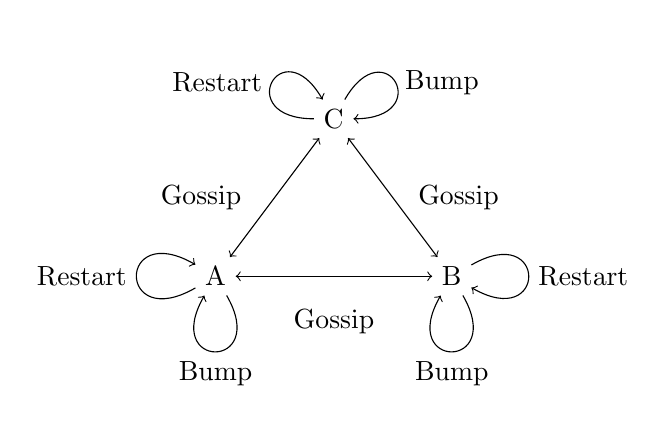
\begin{tikzpicture}
    % Define the nodes
    \node (A) at (0,0) {A};
    \node (B) at (3,0) {B};
    \node (C) at (1.5,2) {C}; % 1.732 is approximately sqrt(3)

    % Draw the edges 
    \path[<->]          (A)  edge   []   node[below=3mm] {Gossip} (B);
    \path[<->]          (A)  edge   []   node[left=3mm] {Gossip} (C);
    \path[<->]          (B)  edge   []   node[right=2mm] {Gossip} (C);

    \path[->]           (A) edge [in=150, out=210, loop, looseness=10] node[left] {Restart} (A);
    \path[->]           (A) edge [in=240, out=300, loop, looseness=10] node[below] {Bump} (A);

    \path[->]           (B) edge [in=-30, out=30, loop, looseness=10] node[right] {Restart} (B);
    \path[->]           (B) edge [in=240, out=300, loop, looseness=10] node[below] {Bump} (B);

    \path[->]           (C) edge [in=120, out=180, loop, looseness=10] node[left] {Restart} (C);
    \path[->]           (C) edge [in=0, out=60, loop, looseness=10] node[right] {Bump} (C);
\end{tikzpicture}
\end{center}

\section{Design}

In this chapter, we will implement a simplified gossip model where: 
\begin{itemize}
    \item Each server has a version.
    \item Each server caches the version of all other servers.
    \item A pair of servers are randomly selected to gossip.
    \item A server can restart. Restarting a server clears the server's version cache
    of the other servers.
    \item A server can bump its version.
\end{itemize}

If the gossip protocol works correctly, every server should eventually have
the latest version of all the servers.

\section{Spec}

In gossip protocol, every server needs to remember all its peer's current
version:\\

\begin{tla}
Init ==
    /\ version = [i \in Servers |-> [j \in Servers |-> 0]]
Next ==
    \/ \E i \in Servers:
        /\ Bump(i)
    \/ \E i, j \in Servers:
        /\ Gossip(i, j)
    \/ \E i \in Servers:
        /\ Restart(i)
\end{tla}
\begin{tlatex}
\@x{ Init \.{\defeq}}%
 \@x{\@s{16.4} \.{\land} version \.{=} [ i \.{\in} Servers \.{\mapsto} [ j
 \.{\in} Servers \.{\mapsto} 0 ] ]}%
\@x{ Next \.{\defeq}}%
\@x{\@s{16.4} \.{\lor} \E\, i \.{\in} Servers \.{:}}%
\@x{\@s{20.5} \.{\land} Bump ( i )}%
\@x{\@s{16.4} \.{\lor} \E\, i ,\, j \.{\in} Servers \.{:}}%
\@x{\@s{20.5} \.{\land} Gossip ( i ,\, j )}%
\@x{\@s{16.4} \.{\lor} \E\, i \.{\in} Servers \.{:}}%
\@x{\@s{20.5} \.{\land} Restart ( i )}%
\end{tlatex}
\newline

The \textit{Init} formula simply declares the version to be a two-dimensional array
with all elements initialized to 0. \textit{Next} allows either bumping the version
of a server, picking a pair of servers to gossip, or restarting a server.\newline

The following defines these steps:\newline

\begin{tla}
Gossip(i, j) == 
    LET 
        Max(a, b) == IF a > b THEN a ELSE b
        updated == [k \in Servers |-> Max(version[i][k], version[j][k])]
        version_a == [version EXCEPT ![i] = updated]
        version_ab == [version_a EXCEPT ![j] = updated]
    IN 
        /\ version' = version_ab 
\end{tla}
\begin{tlatex}
\@x{ Gossip ( i ,\, j ) \.{\defeq}}%
\@x{\@s{16.4} \.{\LET}}%
 \@x{\@s{32.8} Max ( a ,\, b ) \.{\defeq} {\IF} a \.{>} b \.{\THEN} a
 \.{\ELSE} b}%
 \@x{\@s{32.8} updated \.{\defeq} [ k \.{\in} Servers \.{\mapsto} Max (
 version [ i ] [ k ] ,\, version [ j ] [ k ] ) ]}%
 \@x{\@s{32.8} version\_a \.{\defeq} [ version {\EXCEPT} {\bang} [ i ] \.{=}
 updated ]}%
 \@x{\@s{32.8} version\_ab \.{\defeq} [ version\_a {\EXCEPT} {\bang} [ j ]
 \.{=} updated ]}%
\@x{\@s{16.4} \.{\IN}}%
\@x{\@s{32.8} \.{\land} version \.{'} \.{=} version\_ab}%
\end{tlatex}
\newline

When two servers gossip, they gossip about all the servers (including themselves)
and update both of their version cache with the more up-to-date entry between
the two. The \textit{LET..IN} syntax enables local macro definition. In this
example, we use temporary variables defined inside \textit{LET}, and update the
primed variable inside the \textit{IN} clause.\newline

\begin{tla}
Bump(i) == 
    /\ version[i][i] # MaxVersion 
    /\ version' = [version EXCEPT ![i] = [k \in Servers |-> 
        IF i # k THEN version[i][k] ELSE version[i][k] + 1]]
\end{tla}
\begin{tlatex}
\@x{ Bump ( i ) \.{\defeq}}%
\@x{ \.{\land} version [ i ] [ i ] \.{\neq} MaxVersion}%
 \@x{ \.{\land} version \.{'} \.{=} [ version {\EXCEPT} {\bang} [ i ] \.{=} [
 k \.{\in} Servers \.{\mapsto}}%
 \@x{\@s{4.1} {\IF} i \.{\neq} k \.{\THEN} version [ i ] [ k ] \.{\ELSE}
 version [ i ] [ k ] \.{+} 1 ] ]}%
\end{tlatex}
\newline

\textit{Bump} only increments the version if the server hasn't made it to
\textit{MaxVersion}. When the Server bumps the version, it only bumps its
version and keeps all other versions in its version cache as is.\\
\begin{tla}
Restart(i) == 
    /\ version' = [version EXCEPT ![i] = [k \in Servers |-> 
        IF i # k THEN 0 ELSE version[i][i]]]
\end{tla}
\begin{tlatex}
\@x{ Restart ( i ) \.{\defeq}}%
 \@x{\@s{16.4} \.{\land} version \.{'} \.{=} [ version {\EXCEPT} {\bang} [ i ]
 \.{=} [ k \.{\in} Servers \.{\mapsto}}%
 \@x{\@s{20.5} {\IF} i \.{\neq} k \.{\THEN} 0 \.{\ELSE} version [ i ] [ i ] ]
 ]}%
\end{tlatex}
\newline

Upon \textit{Restart}, a server reloads from its local storage (so its version
persists), but the server needs to re-learn the cluster status (all other
entries in its version cache are wiped).\\

\section{Safety}

One safety property is to confirm \textit{all} version values are within bounds:\\
\begin{tla}
Safety == 
    \A i, j \in Servers: 
       /\ version[i][j] >= 0 
       /\ version[i][j] <= MaxVersion
\end{tla}
\begin{tlatex}
\@x{ Safety \.{\defeq}}%
\@x{\@s{16.4} \A\, i ,\, j \.{\in} Servers \.{:}}%
\@x{\@s{16.4} \.{\land} version [ i ] [ j ] \.{\geq} 0}%
\@x{\@s{16.4} \.{\land} version [ i ] [ j ] \.{\leq} MaxVersion}%
\end{tlatex}
\\

This can be read as: for all possible pairs of servers i and j, the value of
\textit{version[i][j]} must be within 0 and \textit{MaxVersion}, inclusive.

\section{Liveness}

\textit{Spec} defines three actions: \textit{Bump}, \textit{Restart},
\textit{Gossip}. Without any fairness description, \textit{Any} permutation of
these actions are allowed by \textit{Spec}, including:
\begin{itemize}
    \item Restart, Restart, Restart,...
    \item Restart, Gossip, Restart, Gossip, ... 
    \item Gossip, Gossip, Gossip, ... 
\end{itemize}

Some of these are not of interest, for example, the cluster is stuck in a
loop where everyone is constantly restarting. In the gossip protocol, we are
interested in verifying the cluster over time converges towards higher version
value for all servers. This means we need to make sure \textit{Bump} is
guaranteed to be called under some circumstances. This is where the fairness
description comes in. To ensure \textit{Bump} is always called:\\

\begin{tla}
Spec ==
  /\ Init
  /\ [][Next]_vars
  /\ WF_vars(Next)
  /\ \A i \in Servers: 
    WF_vars(Bump(i))
\end{tla}
\begin{tlatex}
\@x{ Spec \.{\defeq}}%
\@x{\@s{8.2} \.{\land} Init}%
\@x{\@s{8.2} \.{\land} {\Box} [ Next ]_{ vars}}%
\@x{\@s{8.2} \.{\land} {\WF}_{ vars} ( Next )}%
\@x{\@s{8.2} \.{\land} \A\, i \.{\in} Servers \.{:}}%
\@x{\@s{16.4} {\WF}_{ vars} ( Bump ( i ) )}%
\end{tlatex}
\\

The model checker explores all possible transitions permitted by \textit{Spec}, 
including calling any subset of actions repeatedly.  Fairness description
guarantees that if the enabling condition of an action is true, the action will
be taken. If the system is trapped in a \textit{Restart} and \textit{Gossip}
loop when \textit{Bump} can be called, specifying fairness for \textit{Bump}
ensures \textit{Bump} is called, breaking the loop.\\

With \textit{Spec} ensuring the system always migrate towards higher version
number, we can now define the Liveness property:\\

\begin{tla}
Liveness == 
    \E i, j \in Servers: 
        /\ i # j
        /\ []<>(/\ version[i][i] = MaxVersion
                /\ version[i][j] = MaxVersion
                /\ version[j][i] = MaxVersion
                /\ version[j][j] = MaxVersion)
\end{tla}
\begin{tlatex}
\@x{ Liveness \.{\defeq}}%
\@x{\@s{16.4} \E\, i ,\, j \.{\in} Servers \.{:}}%
\@x{\@s{16.4} \.{\land} i \.{\neq} j}%
 \@x{\@s{16.4} \.{\land} {\Box} {\Diamond} ( \.{\land} version [ i ] [ i
 ]\@s{4.10} \.{=} MaxVersion}%
\@x{\@s{20.5} \.{\land} version [ i ] [ j ] \.{=} MaxVersion}%
\@x{\@s{20.5} \.{\land} version [ j ] [ i ] \.{=} MaxVersion}%
\@x{\@s{20.5} \.{\land} version [ j ] [ j ] \.{=} MaxVersion )}%
\end{tlatex}
\\

The $\Box\Diamond$ represents \textit{always eventually}. The liveness condition
specifies that there exists a pair of Servers such that both of them
\textit{always eventually} make it to \textit{MaxVersion} and have
\textit{Gossip} with each other.\\

Since \textit{Spec} permits \textit{Restart} to be called anytime, a liveness
property where \textit{all} Servers are up-to-date cannot be true. The model
checker can always \textit{Restart} one of the Servers before this property is
met.\\

Likewise, replacing \textit{always eventually} with \textit{eventually always}
($\Diamond\Box$) also fails. $\Diamond\Box$ checks that once the system
\textit{eventually} enters a specified state, it \textit{always} remains in that
state. This cannot be true as the liveness condition is transient, since the
model checker can always disturb any condition with a \textit{Restart}.\\

For a more comprehensive discussion of fairness, please refer to
Chapter~\ref{chap:fairness}.

% \end{document}

